\documentclass[../main]{subfiles}
\begin{document}

\chapter{DSP 数据采集}%
\label{cha:ad}

\section{实验要求}%
\label{sec:\arabic{chapter}requirement}

\begin{Exercise}
  独立完成项目编译、链接、调试的全过程。
\end{Exercise}

\begin{Answer}
  已完成。
\end{Answer}

\begin{Exercise}
  根据范例程序,给出 ADC 的采样频率计算公式,修改 ADC 的采样频率并验证。
\end{Exercise}

\begin{Answer}
  公式如式~\ref{eq:adc}。根据图~\ref{fig:validation}, EPwm1Regs.TBPRD 增大一
  倍,采样频率减小一半,从一个正弦波相邻两波峰之间有 20 个采样点变成 10 个采
  样点。
\end{Answer}

\begin{align}
  \label{eq:adc}
  f = & \frac{\text{TBCLK}}{6\text{TBPRD}}\\
  \label{eq:tbclk}
  \text{TBCLK} = & \frac{\text{SYSCLKOUT}}{\text{HSPCLKDIV} \times \text{CLKDIV}}
\end{align}

\begin{figure}[htbp]
  \centering
  \begin{subfigure}[htbp]{0.45\linewidth}
    \centering
    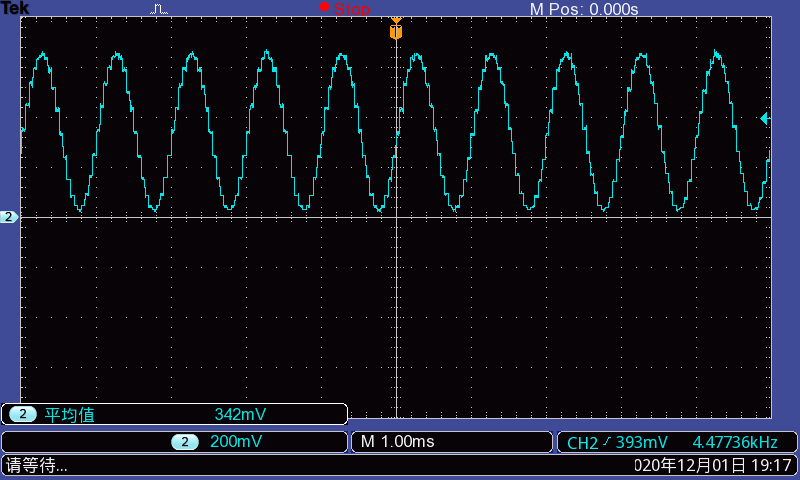
\includegraphics[
      width = \linewidth,
    ]{images/208.png}
    \caption{EPwm1Regs.TBPRD = 208;}%
    \label{fig:208}
  \end{subfigure}
  \quad
  \begin{subfigure}[htbp]{0.45\linewidth}
    \centering
    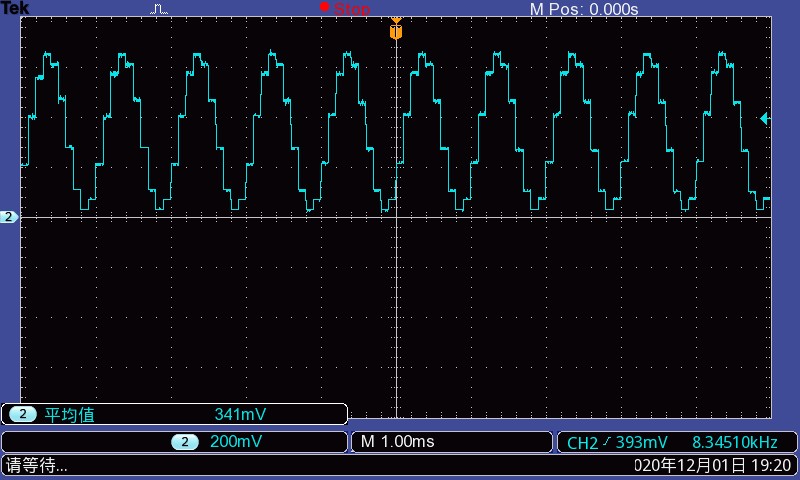
\includegraphics[
      width = \linewidth,
    ]{images/417.png}
    \caption{EPwm1Regs.TBPRD = 417;}%
    \label{fig:417}
  \end{subfigure}
  \caption{验证}%
  \label{fig:validation}
\end{figure}

\begin{Exercise}
  指出波形数据保存的空间地址,并以图形方式显示采集的信号波形,并保存,附在实
  验报告中。
\end{Exercise}

\begin{Answer}
  根据程序~\ref{lst:adc},代码保存在数组 SampleTable1 。结果见
  图~\ref{fig:adc}和图~\ref{fig:validation}。
\end{Answer}

\begin{listing}[htbp]
  \centering
\begin{langPyOne}[c][firstnumber = 348]{code/LAB11/main.c}
	SampleTable1[i++%1024] = AdcRegs.ADCRESULT1;
\end{langPyOne}
  \caption{模数转换代码}%
  \label{lst:adc}
\end{listing}

\begin{figure}[htbp]
  \centering
  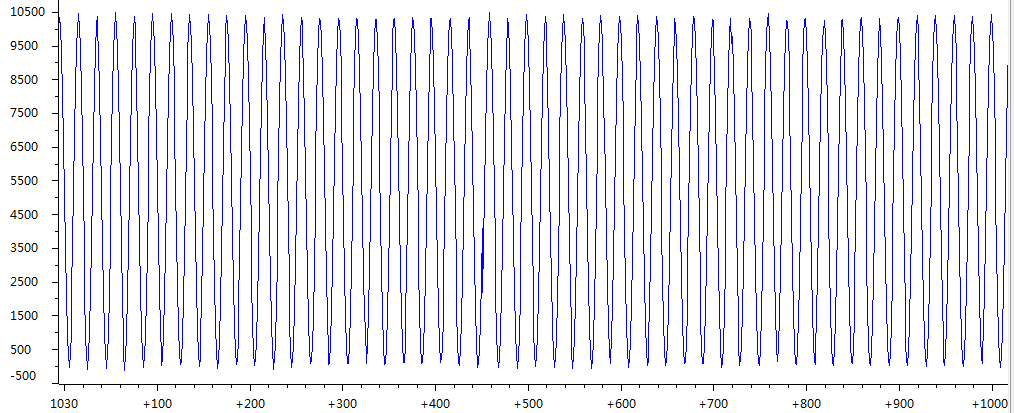
\includegraphics[
    width = 0.8\linewidth,
  ]{images/adc_plot.png}
  \caption{模数转换 CCS 绘图}%
  \label{fig:adc}
\end{figure}

\begin{Exercise}
  利用上述图形,给出验证采样频率的方法,以此验证数据采集程序的正确性。
\end{Exercise}

\begin{Answer}
  以 EPwm1Regs.TBPRD = 208 和输入信号为 1 kHz 正弦波为例。将 EPwm1Regs.TBPRD
  = 208 和 式~\ref{eq:tbclk} 代入式~\ref{eq:adc}可得采样频率 $f$ 为 20 kHz 。

  信号发生器输入信号为 1 kHz 的正弦波。由图~\ref{fig:208} 可得一个正弦波相邻
  两波峰之间有 20 个采样点,所以采样频率 $f$ 为 20 kHz 。
\end{Answer}

\section{实验思考}%
\label{sec:\arabic{chapter}thought}

\begin{Exercise}
  观察输入信号与示波器显示信号、存储器中存储波形信号幅度的差异,解释差异产生
  的原因。
\end{Exercise}

\begin{Answer}
  示波器显示信号幅度小于存储波形信号小于输入信号,原因是信号在传输过程中会有
  衰减。
\end{Answer}

\begin{Exercise}
  除了上述粗略验证 ADC 采样频率以外,思考其他测试采样频率的方法和手段。
\end{Exercise}

\begin{Answer}
  将代码改为程序~\ref{lst:square}后,相邻中断会出现上升沿和下降沿,从而形成方
  波,如图~\ref{fig:square_watch},方波频率的一半是 20 kHz,即为 ADC 采样频率
  。
\end{Answer}

\begin{listing}[htbp]
  \centering
\begin{langPyOne}[c][firstnumber = 352]{code/LAB11/main.c}
	*Da_out=0xffff * (i++%2);
\end{langPyOne}
  \caption{方波代码}%
  \label{lst:square}
\end{listing}

\begin{figure}[htbp]
  \centering
  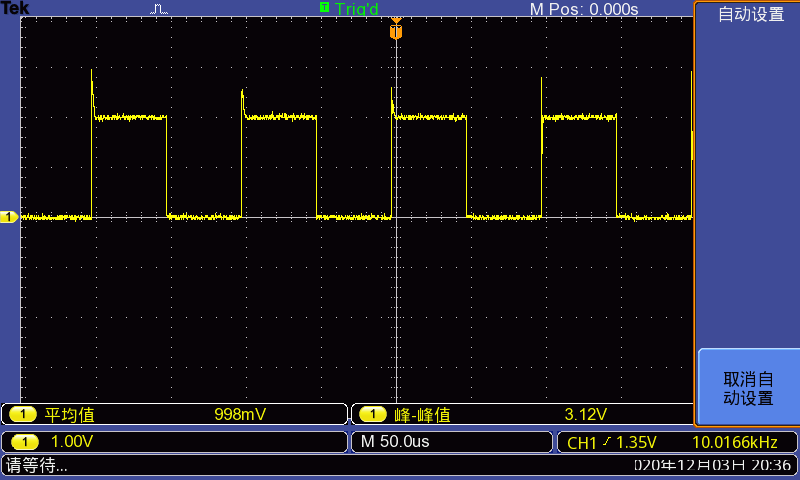
\includegraphics[
    width = 0.6\linewidth,
  ]{images/square_watch.png}
  \caption{方波}%
  \label{fig:square_watch}
\end{figure}

\begin{Exercise}
  除了中断方式,DSP 内核还可以采用查询方式获取 ADC 外设的采样数据。如果采用查
  询方式,则需要查询哪些标志位,试图编程实现。
\end{Exercise}

\begin{Answer}
  将中断改为查询如程序~\ref{lst:consult},查询 ADC\_Result1 ,中断只会在 epwm
  触发中断时改变 Da\_output 其余时间保持不变,如图~\ref{fig:208},而查询会连
  续改变 Da\_output ,所以示波器上会看到完整的正弦波,如
  图~\ref{fig:consult_watch}。
\end{Answer}

\begin{listing}[htbp]
  \centering
\begin{langPyOne}[c][firstnumber = 79]{code/LAB11/main.c}
while(1){
	*Da_out=AdcRegs.ADCRESULT1;
}
\end{langPyOne}
  \caption{查询代码}%
  \label{lst:consult}
\end{listing}

\begin{figure}[htbp]
  \centering
  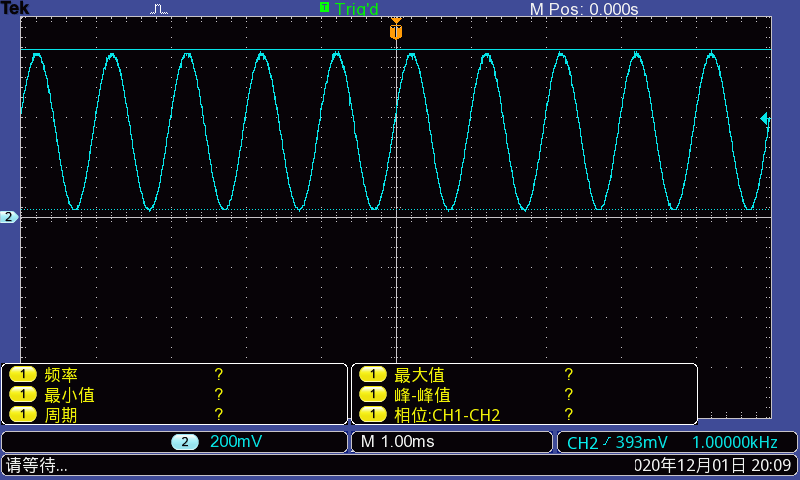
\includegraphics[
    width = 0.8\linewidth,
  ]{images/consult_watch.png}
  \caption{查询}%
  \label{fig:consult_watch}
\end{figure}

\begin{Exercise}
  如何将存储的采样数据保存到数据文件中,并利用动态有效位 ENOB 测试方法分析实
  验平台数据采集的性能。
\end{Exercise}

\begin{Answer}
  在 CCS 绘图窗口右击,在弹出菜单中选择 Data 、 Export All... ,输入文件名再
  选择保存即可。利用 \url{data/enob.csv} 绘制出的波形见图~\ref{fig:enob}。

  动态有效位代码见程序~\ref{lst:enob}。动态有效位为4.7202。
\end{Answer}

\begin{figure}[htbp]
  \centering
  \begin{subfigure}[htbp]{0.45\linewidth}
    \centering
    \includegraphics[
      width = \linewidth,
    ]{figures/t.pdf}
    \caption{时域}%
    \label{fig:t}
  \end{subfigure}
  \quad
  \begin{subfigure}[htbp]{0.45\linewidth}
    \centering
    \includegraphics[
      width = \linewidth,
    ]{figures/f.pdf}
    \caption{频域}%
    \label{fig:f}
  \end{subfigure}
  \caption{波形}%
  \label{fig:enob}
\end{figure}

\begin{listing}
  \centering
  \langCVfile[matlab][][matlab]{figures/enob.m}{figures/enob.m}
  \caption{动态有效位}%
  \label{lst:enob}
\end{listing}

\section{实验总结}%
\label{sec:\arabic{chapter}conclusion}

一些需要注意的地方:

\begin{itemize}
  \item 信号发生器必须要按 output 才能使能输出。
  \item 信号发生器接示波器观测时要注意是否良好接触示波器接口的中心。
  \item 因为 Da\_out 是无符号型,如果采样到负数直接输出底部就会被截断,可以将
    信号发生器输出的信号偏移设为峰峰值的一半,或在代码中将 ADC\_Result1 加上
    一个正数。
\end{itemize}

学长留了几个问题作为思考:

\begin{Exercise}
  如程序~\ref{lst:da},Da\_freq 被赋值了 2 次,第一次赋值不会因为第二次而无效
  吗?
\end{Exercise}

\begin{listing}[htbp]
  \centering
\begin{langPyOne}[c][firstnumber = 74]{code/LAB11/main.c}
    //*Da_freq = 0x0007;   //配置DA频率,32数据,先写高16位,再写低16位
    //*Da_freq = 0xA120;   //50K
    *Da_freq = 0x001E;   //配置DA频率,32数据,先写高16位,再写低16位
    *Da_freq = 0x8480;   //结果要除以10,200K
\end{langPyOne}
  \caption{数模转换频率配置}%
  \label{lst:da}
\end{listing}

\begin{Answer}
  不会。因为如程序~\ref{lst:da_freq},类型 volatile 使变量 Da\_freq 在编译时不
  会被编译器优化掉重复赋值的指令。而 0x201100 是 TMS320F28335 的外部存储区域
  7,在开发板 SEED-DSP28335 上与 DAC7724 相连,先写高 16 位,再写低 16 位才能
  向控制寄存器写入一个完整的 32 位整数去控制数模转换频率。
\end{Answer}

\begin{listing}[htbp]
  \centering
\begin{langPyOne}[c][firstnumber = 21]{code/LAB11/main.c}
volatile Uint16  *Da_freq      = (Uint16 * )0x201100;
\end{langPyOne}
  \caption{数模转换频率声明}%
  \label{lst:da_freq}
\end{listing}

\begin{Exercise}
  将程序改为程序~\ref{lst:adc_cont},程序~\ref{lst:no_mod}会输出
  图~\ref{fig:consult_watch},而程序~\ref{lst:adc}仍会输出
  图~\ref{fig:208};程序~\ref{lst:square}则会输出采样频率恒为 50 kHz 的方波,
  如图~\ref{fig:50},为什么?
\end{Exercise}

\begin{listing}[htbp]
  \centering
\begin{langPyOne}[c][firstnumber = 249]{code/LAB11/main.c}
AdcRegs.ADCTRL1.bit.CONT_RUN=1;  //---- ADC Run at Continuous Conversion Mode//连续转换模式      当接收到EOS信号后,排序器的动作依赖于SEQ-OVRD,如果它等于0,则排序器回到起始状态CONV00;如果它等于1,排序器从当前开始,不要复位
\end{langPyOne}
  \caption{ADC 连续采样}%
  \label{lst:adc_cont}
\end{listing}

\newpage

\begin{listing}[htbp]
  \centering
\begin{langPyOne}[c][firstnumber = 348]{code/LAB11/main.c}
	SampleTable1[i++] = AdcRegs.ADCRESULT1;
  if (i == 1024)
    i = 0;
\end{langPyOne}
  \caption{模数转换代码不取余}%
  \label{lst:no_mod}
\end{listing}

\begin{figure}[htbp]
  \centering
  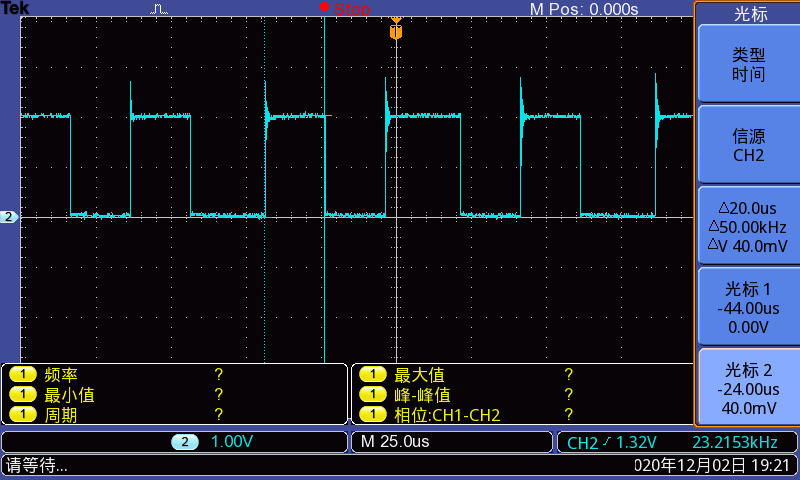
\includegraphics[
    width = 0.8\linewidth,
  ]{images/50.png}
  \caption{方波}%
  \label{fig:50}
\end{figure}

\begin{Answer}
  当 ADC 开启连续转换模式后,采样频率与 epwm 中断频率无关,所以方波恒为 50
  kHz ,图~\ref{fig:208}会因为采样频率过高变成连续的图~\ref{fig:208}。而
  程序~\ref{lst:adc}和程序~\ref{lst:no_mod}等效但因为中断中的求余运算耽搁时间
  过长,所以连续转换模式又因为等待中断完成从而采样频率和 epwm 中断频率一样。
\end{Answer}

\end{document}

